\documentclass[a4paper]{article}

\def\npart {III}
\def\nterm {Michaelmas}
\def\nyear {2017}
\def\nlecturer {P. Sousi}
\def\ncourse {Percolation and Random Walks on Graphs}
\def\nofficial {http://www.statslab.cam.ac.uk/~ps422/percolation.html}

% Imports
\ifx \nextra \undefined
  \usepackage[pdftex,
    hidelinks,
    pdfauthor={Dexter Chua},
    pdfsubject={Cambridge Maths Notes: Part \npart\ - \ncourse},
    pdftitle={Part \npart\ - \ncourse},
  pdfkeywords={Cambridge Mathematics Maths Math \npart\ \nterm\ \nyear\ \ncourse}]{hyperref}
  \title{Part \npart\ - \ncourse}
\else
  \usepackage[pdftex,
    hidelinks,
    pdfauthor={Dexter Chua},
    pdfsubject={Cambridge Maths Notes: Part \npart\ - \ncourse\ (\nextra)},
    pdftitle={Part \npart\ - \ncourse\ (\nextra)},
  pdfkeywords={Cambridge Mathematics Maths Math \npart\ \nterm\ \nyear\ \ncourse\ \nextra}]{hyperref}

  \title{Part \npart\ - \ncourse \\ {\Large \nextra}}
\fi

\author{Lectured by \nlecturer \\\small Notes taken by Dexter Chua}
\date{\nterm\ \nyear}

\usepackage{alltt}
\usepackage{amsfonts}
\usepackage{amsmath}
\usepackage{amssymb}
\usepackage{amsthm}
\usepackage{booktabs}
\usepackage{caption}
\usepackage{enumitem}
\usepackage{fancyhdr}
\usepackage{graphicx}
\usepackage{mathtools}
\usepackage{microtype}
\usepackage{multirow}
\usepackage{pdflscape}
\usepackage{pgfplots}
\usepackage{siunitx}
\usepackage{tabularx}
\usepackage{tikz}
\usepackage{tkz-euclide}
\usepackage[normalem]{ulem}
\usepackage[all]{xy}

\pgfplotsset{compat=1.12}

\pagestyle{fancyplain}
\lhead{\emph{\nouppercase{\leftmark}}}
\ifx \nextra \undefined
  \rhead{
    \ifnum\thepage=1
    \else
      \npart\ \ncourse
    \fi}
\else
  \rhead{
    \ifnum\thepage=1
    \else
      \npart\ \ncourse\ (\nextra)
    \fi}
\fi
\usetikzlibrary{arrows}
\usetikzlibrary{decorations.markings}
\usetikzlibrary{decorations.pathmorphing}
\usetikzlibrary{positioning}
\usetikzlibrary{fadings}
\usetikzlibrary{intersections}
\usetikzlibrary{cd}

\newcommand*{\Cdot}{\raisebox{-0.25ex}{\scalebox{1.5}{$\cdot$}}}
\newcommand {\pd}[2][ ]{
  \ifx #1 { }
    \frac{\partial}{\partial #2}
  \else
    \frac{\partial^{#1}}{\partial #2^{#1}}
  \fi
}

% Theorems
\theoremstyle{definition}
\newtheorem*{aim}{Aim}
\newtheorem*{axiom}{Axiom}
\newtheorem*{claim}{Claim}
\newtheorem*{cor}{Corollary}
\newtheorem*{defi}{Definition}
\newtheorem*{eg}{Example}
\newtheorem*{fact}{Fact}
\newtheorem*{law}{Law}
\newtheorem*{lemma}{Lemma}
\newtheorem*{notation}{Notation}
\newtheorem*{prop}{Proposition}
\newtheorem*{thm}{Theorem}

\renewcommand{\labelitemi}{--}
\renewcommand{\labelitemii}{$\circ$}
\renewcommand{\labelenumi}{(\roman{*})}

\let\stdsection\section
\renewcommand\section{\newpage\stdsection}

% Strike through
\def\st{\bgroup \ULdepth=-.55ex \ULset}

% Maths symbols
\newcommand{\bra}{\langle}
\newcommand{\ket}{\rangle}

\newcommand{\N}{\mathbb{N}}
\newcommand{\Z}{\mathbb{Z}}
\newcommand{\Q}{\mathbb{Q}}
\renewcommand{\H}{\mathbb{H}}
\newcommand{\R}{\mathbb{R}}
\newcommand{\C}{\mathbb{C}}
\newcommand{\Prob}{\mathbb{P}}
\renewcommand{\P}{\mathbb{P}}
\newcommand{\E}{\mathbb{E}}
\newcommand{\F}{\mathbb{F}}
\newcommand{\cU}{\mathcal{U}}
\newcommand{\RP}{\mathbb{RP}}
\newcommand{\CP}{\mathbb{CP}}

\newcommand{\ph}{\,\cdot\,}

\DeclareMathOperator{\sech}{sech}
\DeclareMathOperator{\cosech}{cosech}
\DeclareMathOperator{\cosec}{cosec}

\DeclareMathOperator{\covol}{covol}
\DeclareMathOperator{\vol}{vol}

\let\Im\relax
\let\Re\relax
\DeclareMathOperator{\Im}{Im}
\DeclareMathOperator{\Re}{Re}
\DeclareMathOperator{\im}{im}
\DeclareMathOperator{\image}{image}
\DeclareMathOperator{\Ann}{Ann}

\DeclareMathOperator*{\res}{res}
\DeclareMathOperator{\Res}{Res}
\DeclareMathOperator{\Ind}{Ind}

\DeclareMathOperator{\tr}{tr}
\DeclareMathOperator{\diag}{diag}
\DeclareMathOperator{\rank}{rank}
\DeclareMathOperator{\card}{card}
\DeclareMathOperator{\spn}{span}
\DeclareMathOperator{\adj}{adj}

\DeclareMathOperator{\erf}{erf}
\DeclareMathOperator{\erfc}{erfc}

\DeclareMathOperator{\ord}{ord}
\DeclareMathOperator{\Sym}{Sym}

\DeclareMathOperator{\sgn}{sgn}
\DeclareMathOperator{\orb}{orb}
\DeclareMathOperator{\stab}{stab}
\DeclareMathOperator{\ccl}{ccl}

\DeclareMathOperator{\lcm}{lcm}
\DeclareMathOperator{\hcf}{hcf}

\DeclareMathOperator{\Int}{Int}
\DeclareMathOperator{\id}{id}

\DeclareMathOperator{\betaD}{beta}
\DeclareMathOperator{\gammaD}{gamma}
\DeclareMathOperator{\Poisson}{Poisson}
\DeclareMathOperator{\binomial}{binomial}
\DeclareMathOperator{\multinomial}{multinomial}
\DeclareMathOperator{\Bernoulli}{Bernoulli}
\DeclareMathOperator{\like}{like}

\DeclareMathOperator{\var}{var}
\DeclareMathOperator{\cov}{cov}
\DeclareMathOperator{\bias}{bias}
\DeclareMathOperator{\mse}{mse}
\DeclareMathOperator{\corr}{corr}

\DeclareMathOperator{\otp}{otp}
\DeclareMathOperator{\dom}{dom}

\DeclareMathOperator{\Root}{Root}
\DeclareMathOperator{\supp}{supp}
\DeclareMathOperator{\rel}{rel}
\DeclareMathOperator{\Hom}{Hom}
\DeclareMathOperator{\Aut}{Aut}
\DeclareMathOperator{\Gal}{Gal}
\DeclareMathOperator{\Mat}{Mat}
\DeclareMathOperator{\End}{End}
\DeclareMathOperator{\Char}{char}
\DeclareMathOperator{\ev}{ev}
\DeclareMathOperator{\St}{St}
\DeclareMathOperator{\Lk}{Lk}
\DeclareMathOperator{\disc}{disc}
\DeclareMathOperator{\Isom}{Isom}
\DeclareMathOperator{\length}{length}
\DeclareMathOperator{\energy}{energy}
\DeclareMathOperator{\area}{area}
\DeclareMathOperator{\Syl}{Syl}
\DeclareMathOperator{\cl}{cl}
\DeclareMathOperator{\fix}{fix}

\newcommand{\GL}{\mathrm{GL}}
\newcommand{\SL}{\mathrm{SL}}
\newcommand{\PGL}{\mathrm{PGL}}
\newcommand{\PSL}{\mathrm{PSL}}
\newcommand{\PSU}{\mathrm{PSU}}
\newcommand{\Or}{\mathrm{O}}
\newcommand{\SO}{\mathrm{SO}}
\newcommand{\U}{\mathrm{U}}
\newcommand{\SU}{\mathrm{SU}}

\renewcommand{\d}{\mathrm{d}}
\newcommand{\D}{\mathrm{D}}

\tikzset{->/.style = {decoration={markings,
                                  mark=at position 1 with {\arrow[scale=2]{latex'}}},
                      postaction={decorate}}}
\tikzset{<-/.style = {decoration={markings,
                                  mark=at position 0 with {\arrowreversed[scale=2]{latex'}}},
                      postaction={decorate}}}
\tikzset{<->/.style = {decoration={markings,
                                   mark=at position 0 with {\arrowreversed[scale=2]{latex'}},
                                   mark=at position 1 with {\arrow[scale=2]{latex'}}},
                       postaction={decorate}}}
\tikzset{->-/.style = {decoration={markings,
                                   mark=at position #1 with {\arrow[scale=2]{latex'}}},
                       postaction={decorate}}}
\tikzset{-<-/.style = {decoration={markings,
                                   mark=at position #1 with {\arrowreversed[scale=2]{latex'}}},
                       postaction={decorate}}}

\tikzset{circ/.style = {fill, circle, inner sep = 0, minimum size = 3}}
\tikzset{mstate/.style={circle, draw, blue, text=black, minimum width=0.7cm}}

\definecolor{mblue}{rgb}{0.2, 0.3, 0.8}
\definecolor{morange}{rgb}{1, 0.5, 0}
\definecolor{mgreen}{rgb}{0.1, 0.4, 0.2}
\definecolor{mred}{rgb}{0.5, 0, 0}

\def\drawcirculararc(#1,#2)(#3,#4)(#5,#6){%
    \pgfmathsetmacro\cA{(#1*#1+#2*#2-#3*#3-#4*#4)/2}%
    \pgfmathsetmacro\cB{(#1*#1+#2*#2-#5*#5-#6*#6)/2}%
    \pgfmathsetmacro\cy{(\cB*(#1-#3)-\cA*(#1-#5))/%
                        ((#2-#6)*(#1-#3)-(#2-#4)*(#1-#5))}%
    \pgfmathsetmacro\cx{(\cA-\cy*(#2-#4))/(#1-#3)}%
    \pgfmathsetmacro\cr{sqrt((#1-\cx)*(#1-\cx)+(#2-\cy)*(#2-\cy))}%
    \pgfmathsetmacro\cA{atan2(#2-\cy,#1-\cx)}%
    \pgfmathsetmacro\cB{atan2(#6-\cy,#5-\cx)}%
    \pgfmathparse{\cB<\cA}%
    \ifnum\pgfmathresult=1
        \pgfmathsetmacro\cB{\cB+360}%
    \fi
    \draw (#1,#2) arc (\cA:\cB:\cr);%
}
\newcommand\getCoord[3]{\newdimen{#1}\newdimen{#2}\pgfextractx{#1}{\pgfpointanchor{#3}{center}}\pgfextracty{#2}{\pgfpointanchor{#3}{center}}}

\def\Xint#1{\mathchoice
   {\XXint\displaystyle\textstyle{#1}}%
   {\XXint\textstyle\scriptstyle{#1}}%
   {\XXint\scriptstyle\scriptscriptstyle{#1}}%
   {\XXint\scriptscriptstyle\scriptscriptstyle{#1}}%
   \!\int}
\def\XXint#1#2#3{{\setbox0=\hbox{$#1{#2#3}{\int}$}
     \vcenter{\hbox{$#2#3$}}\kern-.5\wd0}}
\def\ddashint{\Xint=}
\def\dashint{\Xint-}


\renewcommand\L{\mathbb{L}}
\newcommand\Pci[1]{\P_{#1}(|\mathcal{C}(0)| = \infty)}
\begin{document}
\maketitle
{\small
\setlength{\parindent}{0em}
\setlength{\parskip}{1em}

A phase transition means that a system undergoes a radical change when a continuous parameter passes through a critical value. We encounter such a transition every day when we boil water. The simplest mathematical model for phase transition is percolation. Percolation has a reputation as a source of beautiful mathematical problems that are simple to state but seem to require new techniques for a solution, and a number of such problems remain very much alive. Amongst connections of topical importance are the relationships to so-called Schramm--Loewner evolutions (SLE), and to other models from statistical physics. The basic theory of percolation will be described in this course with some emphasis on areas for future development.

Our other major topic includes random walks on graphs and their intimate connection to electrical networks; the resulting discrete potential theory has strong connections with classical potential theory. We will develop tools to determine transience and recurrence of random walks on infinite graphs. Other topics include the study of spanning trees of connected graphs. We will present two remarkable algorithms to generate a uniform spanning tree (UST) in a finite graph $G$ via random walks, one due to Aldous-Broder and another due to Wilson. These algorithms can be used to prove an important property of uniform spanning trees discovered by Kirchhoff in the 19th century: the probability that an edge is contained in the UST of $G$, equals the effective resistance between the endpoints of that edge.

\subsubsection*{Pre-requisites}
There are no essential pre-requisites beyond probability and analysis at undergraduate levels, but a familiarity with the measure-theoretic basis of probability will be helpful.
}
\tableofcontents

\setcounter{section}{-1}
\section{Introduction}
The course is naturally divided into two parts --- percolation, and random walks on graphs. Percolation is one of the simplest models that experience phase transition --- an abrupt change in quantitative feature due to a continuous change of a parameter. Examples include the boiling of water, and the loss of long-range correlation in magnets when temperature increases.

For example, consider an $n \times n$ lattice connected by edges:
\begin{center}
  \begin{tikzpicture}
    \draw (0, 0) rectangle (6, 6);
    \foreach \x in {1,2,3}{
      \draw (\x, 0) -- (\x, 6);
      \draw (0, \x) -- (6, \x); % draw nodes as well
    }
  \end{tikzpicture}
\end{center}
We now fix some $p \in [0, 1]$, and for each edge in the graph, we either keep it or remove it with probability $p$. We can define, for example, the quantity $f_n(p)$, the probability that there is an left-to-right crossing of open edges: % example

For example, we have $f_n(0) = 0$ and $f_n(1) = 1$.

How about $p = \frac{1}{2}$? ``By symmetry'', this must be $\frac{1}{2}$. To see this, we consider the \term{dual lattice}, where we put a vertex in the middle of each square, and put an edge between squares that share a common edge. This is again isomorphic to $\Z^2$. We can do the same procedure with the dual lattice. We see that if there is a left-right crossing of open edges, then there cannot be a top-bottom crossing in the dual graph. But since the two graphs are isomorphic, we are done. % Explain this much better

This is a very important property that is only true in $2$ dimensions. We shall see later that a lot of things we can figure out in $2$ dimensions cannot be extended to higher dimensions.

What about other values of $p$? We might think it should be linear, but that is not the case. If $n$ is large, then the graph looks approximately like

% show example

As $n \to \infty$, this converges to the step function:

% insert example

Now suppose we do a percolation, and we obtain a graph. Suppose this graph is such that $0$ is in an infinite component, i.e.\ $0$ is connected to $\infty$. But we want to know more about the properties of this resulting graph. One way to do so is to perform a random walk on this graph, and see what we can say about this graph. Questions we can ask involve hitting times or transience or recurrence.

In IB Markov Chains, we proved the null recurrence of a random walk on $\Z^2$ by rather direct means. Here we are going to use a rather different approach, where we think of our graph as an electric network. We can then interpret the original question in terms of properties of the electric circuits, which provides powerful tools to understand random walks.

We will also look at the theory of uniform spanning trees, and how they connect to electric networks.

\section{Percolation}
There are two models of percolation --- \term{bond percolation} and \term{site percolation}. In this course, we will focus on bond percolation, but we will look at site percolation in the example sheets.

The very basic set up of percolation theory involves picking a \term{graph} $G = (V, E)$, where \term{$V$} is the set of \term{vertices} and \term{$E$} is the set of \term{edges}. We also pick a \term{percolation probability} $p \in [0, 1]$. For each edge $e \in E$, we keep it with probability $p$ and throw it with probability $1 - p$. In the first case, we say the edge is \emph{open}\index{open edge}\index{edge!open}, and in the latter, we say it is \emph{closed}\index{closed edge}\index{edge!closed}.

More precisely, we define the probability space to be $\Omega= \{0, 1\}^E$, where $0$ denotes a closed edge and $1$ denotes an open one (in the case of site percolation, we have $\Omega = \{0, 1\}^V$). We endow $\Omega$ with the $\sigma$-algebra generated by \term{cylinder sets}
\[
  \{\omega \in \Omega: \omega(e) = x_e \text{ for all }e \in A\},
\]
where $A$ is a finite set and $x_e \in \{0, 1\}$ for all $e$. In other words, this is the product $\sigma$-algebra. As probability measure, we take the product measure $\P_p$, i.e.\ every edge is $1$ with probability $p$ and $0$ with probability $1 - p$. We will write \index{$\eta_p$}$\eta_p \in \{0, 1\}^E$ for the state of the system.

Now what can we say about the graph resulting from this process? One question we may ask is if we can connect two points in the graphs via the edges that remain. To further the discussion, we introduce some notation.

\begin{notation}
  We write \term{$x \leftrightarrow y$} if there is an open path of edges from $x$ to $y$.
\end{notation}

\begin{notation}
  We write $\mathcal{C}(x) = \{y \in V: y \leftrightarrow x\}$\index{$\mathcal{C}(x)$}, the \term{cluster} of $x$.
\end{notation}

\begin{notation}
  We write $x \leftrightarrow \infty$ if $|\mathcal{C}(x)| = \infty$.
\end{notation}

From now on, we shall take $G = \L^d = (\Z^d, E(\Z^d))$, the $d$-dimensional integer lattice.\index{$\L^d$} Then by translation invariance, $|\mathcal{C}(x)|$ has the same distribution as $|\mathcal{C}(0)|$ for all $x$. We now introduce a key piece of notation:
\begin{defi}[$\theta(p)$]\index{$\theta_p$}
  We define $\theta(p) = \P_p(|\mathcal{C}(0)| = \infty)$.
\end{defi}

Most of the questions we ask surround this $\theta(p)$. We first make the most elementary observations:
\begin{eg}
  $\theta(0) = 0$ and $\theta(1) = 1$.
\end{eg}

A natural question to ask is then if we can find $p \in (0, 1)$ such that $\theta(p) > 0$. But even before answering that question, we can ask a more elementary one --- is $\theta$ an increasing function of $p$?

Intuitively, it must be. And we can prove it. The proof strategy is known as \term{coupling}. We have already seen coupling in IB Markov Chains, where we used it to prove the convergence to the invariant distribution under suitable conditions. Here we are going to couple all percolation processes for different values of $P$.

\begin{lemma}
  $\theta$ is an increasing function of $p$.
\end{lemma}

\begin{proof}
  We let $(U(e))_{e \in E(\Z^d)}$ be iid $U[0, 1]$ random variables. For each $p \in [0, 1]$, we define
  \[
    \eta_p(e) =
    \begin{cases}
      1 & U(e) \leq p\\
      0 & \text{otherwise}
    \end{cases}
  \]
  Then $\P(\eta_p(e) = 1) = \P(U(e) < p) = p$. Since the $U(e)$ are independent, so are $\eta_p$. Thus $\eta_p$ has the law of bond percolation with probability $p$.

  Moreover, if $p \leq q$, then $\eta_p(e) \leq \eta_q(e)$. So the result follows.
\end{proof}
Note that this is not only useful as a theoretical tool. If we want to simulate percolation with different probabilities $p$, we can simply generate a set of $U[0, 1]$ variables, and use it to produce a percolation for all $p$.

If we wish, we can provide an abstract definition of what coupling is, but the detailed definition is not of much practical use:
\begin{defi}[Coupling]\index{coupling}
  Let $\mu$ and $\nu$ be two probability measures on (potentially) different probability spaces. A \emph{coupling} is a pair of random variables $(X, Y)$ defined on the same probability space such that the marginal distribution of $X$ is $\mu$ and the marginal distribution of $Y$ is $\nu$.
\end{defi}

%The obvious first question to ask is then:
%\begin{question}
%  Is there $p \in (0, 1)$ such that $\theta(p) > 0$?
%\end{question}
%
%In the degenerate case $d = 1$, we immediately see that we have
%\begin{eg}
%  Take $d = 1$. Then for any $p < 1$, we have $\theta(p) = 0$.
%\end{eg}
%
%If $\theta(p)$ is not always zero, then there is an immediate follow-up question we can ask:
%\begin{question}
%  Is $\theta(p)$ increasing?
%\end{question}
%Intuitively, this must be the case, and indeed we will show that it is true.
%
%Finally, a questions we can ask is:
%\begin{question}
%  Suppose $\theta(p) > 0$. Then how many infinite components are there?
%\end{question}
%
%We first answer question $2$. What we are going to use is \emph{coupling}. The definition will look a little abstract, but we will use it a lot, and we shall see how it is useful in practice.

With the lemma, we can make the definition
\begin{defi}[Critical probability]\index{Critical probability}
  We define $p_c(d) = \sup \{p \in [0, 1]: \theta(p) = 0\}$.
\end{defi}

Recall we initially asked whether $\theta(p)$ can be non-zero for $p \in (0, 1)$. We can now rephrase and strengthen this question by asking for the value of $p_c(d)$. There are a lot more questions we can ask about $p_c$ and $\theta(p)$.

For example, we know that $\theta(p)$ is a $C^\infty$ function on $(p_c, 1]$. However, we do not know if $\theta$ is continuous at $p_c$ in $d = 3$. We will see soon that $p_c = \frac{1}{2}$ in $d = 2$, but the exact value of $p_c$ is not known in higher dimensions.

Let's start actually proving things about $p_c$. We previously noted that
\begin{prop}
  $p_c(1) = 1$.
\end{prop}

The first actually interesting theorem is the following:
\begin{thm}
  For all $d \geq 2$, we have $p_c(d) \in (0, 1)$.
\end{thm}

We shall break this up into two natural parts:
\begin{lemma}
  For $d \geq 2$, $p_c(d) > 0$.
\end{lemma}

\begin{proof}
  Write $\Sigma_n$ for the number of open self-avoiding paths of length $n$ starting at $0$. We then note that
  \[
    \P_p(|\mathcal{C}(0)| = \infty) = \P_p(\forall n \geq 1: \Sigma_n \geq 1) = \lim_{n \to \infty} \P_p(\Sigma_n \geq 1) \leq \lim_{n \to \infty} \E_p[\Sigma_n].
  \]
  We can now compute $\E_p[\Sigma_n]$. The point is that expectation is linear, which makes this much easier to compute. We let $\sigma_n$ be the number of self-avoiding paths of length $n$ from $0$. Then we simply have
  \[
    \E_p[\Sigma_n] = \sigma_n p^n.
  \]
  We can bound $\sigma_n$ by $2d \cdot (2d - 1)^{n - 1}$, since we have $2d$ choices of the first step, and at most $2d - 1$ choices in each subsequent step. So we have
  \[
    \E_p[\Sigma_n] \leq 2d (2d - 1)^{n - 1} p^n = \frac{2d}{2d - 1} (p(2d - 1))^n.
  \]
  So if $p (2d - 1) < 1$, then $\theta(p) = 0$. So we know that
  \[
    p_c(d) \geq \frac{1}{2d - 1}.\qedhere
  \]
\end{proof}

Let's now talk a bit more about self-avoiding paths. We only needed a very crude bound for the proof, but there is more we can say. Again, we write \term{$\sigma_n$} for the number of \term{self-avoiding path}\emph{s} of length $n$ starting from $0$.

\begin{lemma}
  We have $\sigma_{n + m} \leq \sigma_n \sigma_m$
\end{lemma}

\begin{proof}
  A self-avoiding path of length $n + m$ can be written as a concatenation of self-avoiding paths of length $n$ starting from $0$ and another one of length $m$.
\end{proof}
Taking the logarithm, we know that $\log \sigma_n$ is a \term{subadditive sequence}.

A rather convenient lemma is
\begin{lemma}[Fekete's lemma]\index{Fekete's lemma}
  If $(a_n)$ is a subadditive sequence of real numbers, then
  \[
    \lim_{n \to \infty} \frac{a_n}{n} = \inf\left\{\frac{a_k}{k}: k \geq 1\right\} \in [-\infty, \infty).
  \]
  In particular, the limit exists.
\end{lemma}

\begin{cor}
  The limit $\lambda = \lim_{n \to \infty} \frac{\log \sigma_n}{n}$ exists.
\end{cor}
Thus, we have
\[
  \sigma_n= e^{n \lambda (1 + o(1))}
\]
as $n \to \infty$. The quantity \index{$\kappa$}$\kappa = e^\lambda$ is the \term{connective constant}. We don't know the value of $\kappa$ for the Euclidean lattice, and the value for the hexagonal lattice has only been found recently:
\begin{thm}[Duminil-Copin, Smirnov] % insert year
  The hexagonal lattice has
  \[
    \kappa_{\mathrm{hex}} = \sqrt{2 + \sqrt{2}}.
  \]
\end{thm}
We can try to say more precisely about how $\sigma_n$ grows.
\begin{conjecture}
  \[
    \sigma_n \approx
    \begin{cases}
      n^{11/32} \kappa^n & d = 2\\
      n^\gamma \kappa^n & d = 3\\
      (\log n)^{1/4} \kappa^n & d = 4
    \end{cases}
  \]
\end{conjecture}

For larger $d$, we have an actual theorem
\begin{thm}[Hara and Slade] % check and year
  For $d \geq 5$, we have
  \[
    \sigma_n \approx \kappa^n
  \]
\end{thm}

We also have a theorem
\begin{thm}[Hammersley and Welsh]
  For all $d \geq 2$, we have
  \[
    \sigma_n \leq C \kappa^n \exp(c' \sqrt{n})
  \]
  for some constants $C$ and $c'$.
\end{thm}

In fact, a better bound was recently found:
\begin{thm}[Hutchcroft]
  For $d \geq 2$, we have
  \[
     \sigma_n \leq C \kappa^n \exp(o(\sqrt{n})).
  \]
\end{thm}
This will be proved in the example sheet. % check

Fixing an $n$, there are only finitely many self-avoiding walks of length $n$. So we can sample such a self-avoiding walk uniformly at random. We would like to study the scaling limit, namely what happens when we increase $n$ while simultaneously shrinking space by a factor of $\frac{1}{\sqrt{n}}$. We would expect the result to tend towards some Brownian-motion-like thing, but we want a more precise description.

It is conjectured that for $d = 2$, the scaling limit is given by $SLE(\frac{8}{3})$.

On the other hand, this was proved for self-avoiding walks on a random surface by Gwynne--Miller. % check

Now let's return to our problem of understanding $p_c(d)$. We have yet to show that it is $ < 1$. To do so, we introduce the notion of a dual lattice.

\begin{defi}[Planar graph]\index{planar graph}\index{graph!planar}
  A graph $G$ is called planar if it can be embedded on the plane in such a way that no two edges cross.
\end{defi}

\begin{defi}[Dual graph]\index{dual graph}\index{graph!dual}
  Let $G$ be a planar graph (which we call the \term{primal graph}\index{graph!primal}). We define the \emph{dual graph} by placing a vertex in each face of $G$, and connecting $2$ vertices if their faces share a boundary edge.
\end{defi}

\begin{eg}
  The dual of $\Z^2$ is isomorphic to $\Z^2$ % insert picture
\end{eg}
The dual lattice will help us prove a lot of properties for percolation in $\Z^2$.

\begin{lemma}
  $p_c(d) < 1$ for all $d \geq 2$.
\end{lemma}

\begin{proof}
  It suffices to show this for $d = 2$, since $\Z^d$ embeds in $\Z^{d + 1}$ for all $d$, and if there is an infinite cluster in $Z^d$, the same is true for $\Z^{d + 1}$

  In order to show that $p_c(2) < 1$, we need to find $\varepsilon, \delta > 0$ such that $\P_p(|\mathcal{C}(0)| < \infty) < 1 - \varepsilon$ for $p < 1 - \delta$.

  Consider the dual of $\Z^2$, and perform bond percolation. We declare an edge of the dual open if it crosses an open edge of $\Z^2$, and closed otherwise.

  Suppose $|\mathcal{C}(0)| < \infty$. This means we can find a closed circuit in the dual lattice, namely the ``boundary'' of $\mathcal{C}(0)$.

  We let $D_n$ be the number of closed dual circuits of length $n$ that surround $0$. So
  \[
    \P_p(|\mathcal{C}(0)| < \infty) = \P_p(\exists n \geq D_n \geq 1) \leq \sum_{n = 4}^\infty \E_p[D_n],
  \]
  using the union bound and Markov's inequality.

  By simple counting, we find that
  \begin{ex}
    Show that the number of dual circuits of length $n$ that contain $0$ is at most $n \cdot 4^n$.
  \end{ex}
  It then follows that
  \[
    \P_p(|\mathcal{C}(0)| < \infty) \leq \sum_{n = 4}^\infty n \cdot 4^n (1 - p)^n.
  \]
  So we find that if $1 - p < \delta$ for a suitable $\delta$, then $\P_p(|\mathcal{C}(0)| < \infty) < 1 - \varepsilon$.
\end{proof}

Now we know that if $p > p_c(d)$, then $\theta(p) > 0$; if $p < p_c(d)$, then $\theta(p) = 0$.

In the first case, it is of course not necessarily the case that with probability $1$, $0$ is connected to $\infty$. However, it turns out it is true that there will almost surely be an infinite cluster, and there is a unique one.

\begin{prop}
  Let $A_\infty$ be the event that there is an infinite cluster.
  \begin{enumerate}
    \item If $\theta(p) = 0$, then $\P_p(A_\infty) = 0$.
    \item If $\theta(p) > 0$, then $\P_p(A_\infty) = 1$.
  \end{enumerate}
\end{prop}

\begin{proof}\leavevmode
  \begin{enumerate}
    \item We have
      \[
        \P_p(A_\infty) = \P_p(\exists x: |\mathcal{C}(x)| = \infty) \leq \sum_{x \in \Z^d} \P_p(|\mathcal{C}(x)| = \infty) = \sum \theta(p) = 0.
      \]
    \item We need to apply the Kolmogorov 0-1 law. Recall that if $X_1, X_2, \ldots$ are independent random variables, and $\mathcal{F}_n = \sigma(X_k: k \geq n)$, $\mathcal{F}_\infty = \bigcap_{n \geq 0} \mathcal{F}_n$. Then $\mathcal{F}_\infty$ is trivial, i.e.\ for all $A \in \mathcal{F}_\infty$, $\P(A) \in \{0, 1\}$.

      So we order the edges of $\Z^d$ as $e_1, e_2, \ldots$ and denote their states $w(e_1), w(e_2), \ldots$. These are iid random varaibles. We certainly have $\P_p(A_\infty) \geq \theta(p) > 0$. So if we can show that $A_\infty \in \mathcal{F}_\infty$, then we are done. But this is clear, since changing the states of a finite number of edges does not affect the occurrence of $A_\infty$.
  \end{enumerate}
\end{proof}

We can make a stronger statement:
\begin{thm}[Burton and Keane] % check
  If $p > p_c$, then there exists a unique infinite cluster with probability $1$.
\end{thm}

\begin{proof}
  Let $N$ be the number of infinite clusters. We need to show that $\P_p(N = 1) = 1$. Now note that $\{N = k\}$ is not in $\mathcal{F}_\infty$ when $k \not= 0, \infty$, since changing a finite number of edges can break up or join together infinite clusters. So the Kolmogorov 0-1 law does not apply.

  However, we do note that $N$ is translation invariant. It is an exercise to show that if $N$ is translation invariant, then $N$ is constant with probability $1$.

  Thus, we know that there is some $k \in \{0, 1, \ldots\} \cup \{\infty\}$ such that $\P_p(N = k) = 1$.

  First of all, we know that $k \not= 0$, since $\theta(p) > 0$. We will exclude $k \geq 2$ and $k = \infty$.

  We first show that we cannot have $2 \leq k < \infty$. Assume that $k < \infty$. We have to show that $k = 1$. We let $B(n) = [-n, n]^d \cap \Z^d$, and let $\partial B(n)$ be its boundary. We know that
  \[
    \P_p(N = k, \text{all $k$ clusters intersect $\partial B(n)$}) \to 1
  \]
  as $n \to \infty$.

  Take an $n$ sufficiently large, such that
  \[
    \P_p(\text{all infinite clusters intersect }\partial B(n)) \geq \frac{1}{2}.
  \]
  We then have
  \[
    \P_p(N = 1) \geq \P_p(\text{all infinite clusters intersect }\partial B(n)\text{ and all edges in $B(n)$ are open})
  \]
  Finally, note that the two events in there are independent, since they involve different edges.

  But the probability that all edges in $B(n)$ are open is just $p^{E(B(n))}$. So
  \[
    \P_p(N = 1) \geq \frac{1}{2} p^{E(B(n))} > 0.
  \]
  So we are done, since $N$ is a constant.

  What remains to be shown is that $k$ has to be finite. Suppose $k$ were infinite, i.e.\ $\P_p(N = \infty) = 1$. The idea of the proof is define what it means for a vertex to be a \emph{trifurcation}. We then prove that $\P_p(0\text{ is a trifurcation}) \geq c > 0$. We next show that the number of trifurcations inside $B(n)$ is $\leq |\partial B(n)|$. These two are contradictory, since the first tells us the expected number of trifurctaions is $O(n^d)$, but the latter shows us it is bounded by $O(n^{d - 1})$.

  We say a vertex $x$ is a \term{trifurcation} if the following three conditions hold:
  \begin{enumerate}
    \item $x$ is in an infinite open cluster $\mathcal{C}_\infty$;
    \item there exist exactly three open edges adjacent to $x$;
    \item $\mathcal{C} \infty \setminus \{x\}$ contains exactly three infinite clusters and no finite ones.
  \end{enumerate}
  This is clearly a translation invariant notion. So $\P_p(0 \text{ is a trifurcation}) = \P_p(x \text{ is a trifurcation})$ for all $x \in \Z^d$.

  \begin{claim}
    $\P_p(0\text{ is a trifurcation})\geq c > 0$.
  \end{claim}
   We let $S(n) = \{x \in \Z^d: \|x\|_1 \leq n\}$. This looks like a diamond. A crucial property of this is that for any $x_1, x_2, x_3 \in \partial S(n)$, there exist three disjoint self-avoiding paths joining $x_i$ to $0$ (exercise!). For each triple $x_1, x_2, x_3$, we fix a set of three such paths, and define
   \[
     J(x_1, x_2, x_3) = \{\text{all edges on these 3 paths are open and everything else inside $S(n)$ is closed}\}.
   \]
   Then
   \[
     \P_p(0 \text{ is a trifurcation}) \geq \P_p(\exists \mathcal{C}_\infty^1, \mathcal{C}_\infty^2, \mathcal{C}_\infty^3 \subseteq \Z^d \setminus S(n) \text{ infinite clusters which intersect $\partial S(n)$ at $x_1, x_2, x_3$, and $J(x_1, x_2, x_3)$} % can have multiple intersections; pick one randomly
   \]
   We can then write this as $\P_p(J(x_1, x_2, x_3) \mid\exists \mathcal{C}_\infty^1, \mathcal{C}_\infty^2, \mathcal{C}_\infty^3 \subseteq \Z\text{ intersecting }\partial S(n)) \times \P_p(\exists \mathcal{C}_\infty^1, \mathcal{C}_\infty^2, \mathcal{C}_\infty^3 \subseteq \Z^d \setminus \partial S(n))$. We can bound the first term by
   \[
     \min(p, 1 - p)^{E(S(n))}.
   \]
   To bound the second probability, we have already assumed that $\P_p(N = \infty) = 1$. So $\P_p(\exists \mathcal{C}_\infty^1, \mathcal{C}_\infty^2, \mathcal{C}_\infty^3 \subseteq \Z^d \setminus S(n)\text{ intersecting }\partial S(n)) \to 1$ as $n \to \infty$. We can then take $n$ large enough such that $\P_p( \cdots ) \geq \frac{1}{2}$. So we have shown that $\P_p(0\text{ is a trifurcation}) \geq c > 0$.

   From this, it follows that
   \[
     \E_p[\text{number of trifurcations inside $B(n)$})] \geq c |B(n)| \sim n^d.
   \]
   So if we can show that the number of trifuractions in $B(n) \leq |\partial B(n)|$, then we arrive at a contradiction, since $|\partial B(n) \sim n^{d - 1}$.

   Indeed, suppose $x_1$ is a trifurcation in $B(n)$. By definition, there exists $3$ open paths to $\partial B(n)$. Let $x_2$ be another trifurcation. Then its paths to the boundary could intersect those of $x_1$, but cannot create a cycle, by definition of a trifurcation.

   For simplicity, we add the rule that when we produce the paths for $x_2$, once we intersect the path of $x_1$, we continue following the path of $x_1$.

   Exploring all trifurcations this way, we obtain a forest inside $B(n)$, and the boundary points will be the leaves of the forest. Now the trifurcations have degree $3$ in this forest. The rest is just combinatorics.
   \begin{claim}
     For any tree, the number of degree $3$ vertices is always less than the number of leaves. % prove this
   \end{claim}
\end{proof}

\subsection{Correlation inequalities}
Suppose again we perform bond percolation. We want to know the probabilities
\[
  \P_p(x \leftrightarrow y \mid u \leftrightarrow v).
\]
Intuitively, we expect this to be greater than $\P_p(x \leftrightarrow y)$, since $u \leftrightarrow v$ tells us there are some open edges around, which is helpful. The proof of this will follow from the FKG inequality.

Again, let $G = (V, E)$ be a graph, let $\Omega = \{0, 1\}^E$, $\mathcal{F}$ the product $\sigma$-algebra, and $\P_p$ the product measure.

\begin{defi}[$\leq$]\index{$\leq$}
  Given $\omega, \omega' \in \Omega$, we write $\omega \leq \omega'$ if $\omega(e) \leq \omega'(e)$ for all $e \in E$.
\end{defi}
This defines a partial order on $\Omega$.

\begin{defi}[Increasing random variable]\index{increasing random variable}\index{random variable!increasing}\index{decreasing random variable}\index{random variable!decreasing}
  A random variable $X$ is increasing if $X(\omega) \leq X(\omega')$ whenever $\omega \leq \omega'$, and is decreasing if $-X$ is increasing
\end{defi}

\begin{defi}[Increasing event]\index{increasing event}\index{event!increasing}\index{event!decreasing}\index{decreasing event}
  An event $A$ is increasing (resp.\ decreasing) if the indicator $1(A)$ is increasing (resp.\ decreasing)
\end{defi}

\begin{eg}
  $\{|\mathcal{C}(0)|= \infty\}$ is an increasing event.
\end{eg}

\begin{thm}
  If $N$ is an increasing random variable and $p_1 \leq p_2$, then
  \[
    \E_{p_1} [N] \leq \E_{p_2} [N],
  \]
  and if an event $A$ is increasing, then
  \[
    \P_{p_1}(A) \leq \P_{p_2}(A).
  \]
\end{thm}

\begin{proof}
  Immediate from coupling.
\end{proof}

\begin{thm}[FKG inequality]\index{FKG inequality} % insert name
  let $X$ and $Y$ be increasing random variables with $\E_p[X^2], \E_p[Y^2] < \infty$. Then
  \[
    \E_p[XY] \geq \E_p[X] \E_p[Y].
  \]
  In particular, if $A$ and $B$ are increasing events, then
  \[
    \P_p(A \cap B) \geq \P_p(A) \P_p(B).
  \]
  Equivalently,
  \[
    \P_p(A \mid B) \geq \P_p(A).
  \]
\end{thm}
This in fact holds on a greater generality than the product measure.

We will actually use the FKG inequality quite a lot.
\begin{proof}
  We assume first that $X$ and $Y$ depend on the state of a finite number of edges. We induct on the number of edges on this number. If $X$ and $Y$ depend on $\omega(e_1)$ only. Then for any $\omega_1, \omega_2 \in \{0, 1\}$, we claim that
  \[
    (X(\omega_1) - X(\omega_2))(Y(\omega_1) - Y(\omega_2)) \geq 0.
  \]
  Indeed, $X$ and $Y$ are both increasing. So if $\omega_1 > \omega_2$, then both terms are positive; if $\omega < \omega_2$, then both terms are negative, and there is nothing to do if they are equal.

  We then have
  \[
    \sum_{\omega_1, \omega_2 \in \{0, 1\}} (X(\omega_1) - X(\omega_2)) (Y(\omega_1) - Y(\omega_2)) \P_p( \omega(e_1) = \omega_1) \P_p(\omega(e_1) = \omega_2) \geq 1.
  \]
  Expanding this, we find that the LHS is $\E_p[XY] - \E_p[X] \E_p[Y]$, and we are done.

  Now suppose the claim holds for $X$ and $Y$ that depend on $n < k$ edges. We shall prove the result when they depend on $k$ edges $\omega(e_1), \ldots, \omega(e_k)$. We have
  \[
    \E_p[XY] = \E_p[\E_p[XY \mid \omega(e_1), \ldots, \omega(e_{k - 1})]].
  \]
  Now after conditioning on $\omega(e_1), \ldots, \omega(e_{k - 1})$, the random variables $X$ and $Y$ become increasing random variables of $\omega(e_k)$. Applying the first step, we get
  \[
    \E_p[X Y \mid \omega(1_, \ldots, \omega(e_{k - 1})] \geq \E_p[X \mid \omega(e_1), \ldots, \omega(e_{k - 1})] \E_p[Y \mid \omega(e_1), \ldots, \omega(e_{k - 1})].
  \]
  But $\E_p[X \mid \omega(e_1), \ldots, \omega(e_{k - 1})]$ is a random variable depending on the edges $e_1, \ldots, e_{k - 1}$, and moreover it is increasing. So applying the induction hypothesis, we obtain
  \[
    \E_p[\E_p[X \mid \omega(e_1), \ldots, \omega(e_{k - 1})] \E_p[Y \mid \omega(e_1), \ldots, \omega(e_{k - 1})]] \geq \E_p[\E_p[X \mid \omega(e_1), \ldots, \omega(e_{k - 1})]] \E_p[\E_p[Y \mid \omega(e_1), \ldots, \omega(e_{k - 1})]]
  \]
  Now suppose $X$ and $Y$ depend on the states of a countable set of edges $e_1, e_2, \ldots$. Let's define
  \begin{align*}
    X_n &= \E_p [X \mid \omega(e_1), \ldots, \omega(e_n)]\\
    Y_n &= \E_p [Y \mid \omega(e_1), \ldots, \omega(e_n)]
  \end{align*}
  Then $X_n$ and $Y_n$ are martingales, and depend only on the states of only finitely many edges. So we know that
  \[
    \E_p[X_n Y_n] \geq \E_p [X_n] \E_p[Y_n] = \E_p[X] \E_p[Y].
  \]
  By the $\mathcal{L}^2$-martingale convergence theorem, $X_n \to X$, $Y_n \to Y$ in $L^2$ and almost surely. So taking the limit $n \to \infty$, we get
  \[
    \E_p[XY] \geq \E_p[X] \E_p[Y].
  \]
\end{proof}

\begin{eg}
  Suppose we perform bond percolation on $\Z^d$. Let $x, y, z, w$ be $4$ vertices and $\{x \leftrightarrow y\}$ and $\{z \leftrightarrow w\}$ disjointly, i.e.\ there are $2$ disjoint paths of open edges, one joining $x$ to $y$ and the other one joining $z$ to $w$.
\end{eg}

We want to formulate this scenario generally:
\begin{defi}[Disjoint occurrence]\index{disjoint occurrence}
  Let $F$ be a set and $\Omega = \{0, 1\}^F$. Let $S \subseteq F$. We define
  \[
    [\omega]_S = \{\omega' \in \Omega: \omega'(e) = \omega(e)\text{ for all }e \in S\}.
  \]
  If $A$ and $B$ are $w$ events, then
  \[
    A \circ B = \{\omega \in \Omega : \exists S \subseteq F\text{ s.t. } [\omega]_S \subseteq A \text{ and } [\omega]_{F\setminus S} \subseteq B\}.
  \]
\end{defi}

\begin{thm}[BK inequality]\index{BK inequality} % van den Berg and Kesten
  Let $F$ be a finite set and $\Omega = \{0, 1\}^F$. Let $A$ and $B$ be $2$ increasing events. Then
  \[
    \P_p(A \circ B) \leq \P_p(A) \P_p(B).
  \]
\end{thm}

\begin{proof}[Proof (Bollob\'as and Leader)]
  We prove by induction on the size $n$ of the set $F$. For $n = 0$, it is trivial.

  Suppose it holds for $n - 1$. We want to show it holds for $n$. For $D \subseteq \{0, 1\}^F$ and $i =0, 1$, set
  \[
    D_i = \{(\omega_1, \ldots, \omega_{n - 1}) : (\omega_1, \ldots, \omega_{n - 1}, i) \in D\}.
  \]
  Let $A, B \subseteq \{0, 1\}^F$, and $C = A \circ B$. We check that
  \[
    C_0 = A_0 \circ B_0,\quad C_1 = (A_0 \circ B_1) \cup (A_1 \circ B_0).
  \]
  Since $A$ and $B$ are increasing, $A_0 \subseteq A_1$ and $B_0 \subseteq B_1$, and $A_i$ and $B_i$ are also increasing events. So
  \begin{align*}
    C_0 &\subseteq (A_0 \circ B_1) \cap  (A_1 \circ B_0)\\
    C_1 &\subseteq A_1 \circ B_1.
  \end{align*}
  By the induction hypothesis, we have
  \begin{align*}
    \P_p(C_0) &= \P_p(A_0 \circ B_0) \leq \P_p(A_0) \P_p(B_0)\\
    \P_p(C_1) &\leq \P_p(A_1 \circ B_1) \leq \P_p(A_1) \P_p(B_1)\\
    \P_p(C_0) + \P_p(C_1) \leq \P_p((A_0 \circ B_1) \cap (A_1 \circ B_0)) + \P_p((A \circ B_1) \cup (A_1 \circ B_0))\\
    &= \P_p(A_0 \circ B_1) + \P_p(A_1 \circ B_0)\\
    &\leq \P_p(A_0) \P_p(B_1) + \P_p(A_1) \P_p(B_0).
  \end{align*}
  Now note that for any $D$, we have
  \[
    \P_p(D) = p \P_p(D_1) + (1 - p) \P_p(D_0).
  \]
  By some black magic, we multipy the first inequality by $(1 - p)^2$, the second by $p^2$ and the third by $p(1 - p)$. This gives
  \[
    p\P_p(C_1) + (1 - p)\P_p(C_0) \leq (p\P_p(A_1) + (!- p)\P_p(A_0))(p\P_p(B_1) + (1 - p) \P_p(B_0)).
  \]
  So we are done.
\end{proof}

It turns out the increasing hypothesis is not necessary:
\begin{thm}[Reimer]
  For all events $A, B$ depending on a finite set, we have $\P_p(A \circ B) \leq \P_p(A) \P_p(B)$.
\end{thm}
But the proof is much harder, and in all the case where we want to apply this, the variables are increasing.

Recall we defined
\[
  \theta(p) = \P_p( |\mathcal{C}(0)| = \infty).
\]
We also define
\[
  \chi(p) = \E_p[|\mathcal{C}(0)|].
\]
If $\chi(p)$ is finite, then of course $\theta(p) = 0$. However, the converse need not hold. So finiteness of $\chi(p)$ is a stronger condition than the vanishing of $\theta(p)$.

Recall that $B(n) = [-n, n]^d \cap \Z^d$. % consnstent notation
\begin{thm}
  If $\chi(p) < \infty$, then there exists a positive constant $c$ such that for all $n \geq 1$,
  \[
    \P_p(0 \leftrightarrow \partial B(n)) \leq e^{-cn}.
  \]
\end{thm}
We will later prove it under the assumption of $p < p_c$. % application of BK inequality

The idea of the proof is that for there to be a path from, say, $0$ to $B(2n)$, the path must hit a point on $\partial B(n)$. So there is a path from $0$ to a point on $\partial B(n)$, and a path from that point to $\partial B(2n)$. Moreover, these two paths are disjoint, which allows us to apply the BK inequality.
\begin{proof}
  Let
  \[
    X_n = \sum_{x \in \partial B(n)} 1(0 \leftrightarrow x).
  \]
  Now consider
  \[
    \sum_{n = 0}^\infty \E[X_n] = \sum_n \sum_{x \in \partial B_n} \P_p(0 \leftrightarrow x) = \sum_{x \in \Z^d} \P_p(0 \leftrightarrow x) = \chi(p).
  \]
  Since $\chi(p)$ is finite, we in particular have $\E_p[X_n] \to 0$ as $n \to \infty$. Take $m$ large enough such that $\E_p[X_m] < \delta < 1$.

  Now we have
  \begin{align*}
    \P_p( 0 \leftrightarrow \partial B_{m + k}) &= \P_p(\exists \in \partial B_m : 0 \leftrightarrow x \text{ and } x \to \partial B_{m + k}\text{ disjointly })\\
    &\leq \sum_{x \in \partial B_m} \P_p(0 \leftrightarrow) \P_p(x \leftrightarrow \partial B_{m + k}) \tag{union bound + BK}\\
    &\leq \sum_{x \in \partial B_m} \P_p(0 \leftrightarrow) \P_p(x \leftrightarrow \partial B_{k}) \tag{trans. inv.}\\
    &\leq \P_p(0 \leftrightarrow B_k) \E_p[X_m].
  \end{align*}
  So for any $n > m$, write $n = qm + r$, where $r \in [0, m - 1]$. Then interating the above result, we have
  \[
    \P_p(0 \leftrightarrow \partial B_n) \leq \P_p(0 \leftrightarrow B_{mq}) \leq \delta^q \leq \delta^{-1 + \frac{n}{m}} \leq e^{-cn}.
  \]
\end{proof}

We know that $\theta(p)$ is an increasing function of $p$. But at what rate does it increase? In other words, we want to look at $\frac{\d \theta}{\d p}$, if this even makes sense. For these, we need the notion of a pivotal edge. Suppose the cluster of $0$ looks as follows:

\begin{center}
  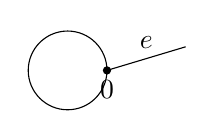
\begin{tikzpicture}
    \node [circ] at (0, 0) {};
    \node [below] at (0, 0) {$0$};
    \draw (-0.5, 0) circle [radius=0.5];
    \draw (0, 0) -- (1, 0.3) node [pos=0.5, above] {$e$}; % some random paths spawning from this edge
  \end{tikzpicture}
\end{center}
Here if we remove the single edge $e$, then we no longer have an infinite cluster.

\begin{defi}[Pivotal edge]\index{pivotal edge}
  Let $A$ be an event and $w$ a percolation configuration. The edge $e$ is \emph{pivotal} for $(A, w)$ if $1(\omega \in A) \not= 1(\omega' \in A)$, where $\omega'(f) = \omega(f)$ for all $f \not= e$, and $\omega'(e) \not= \omega(e)$.
  \[
    \{e \text{ is pivotal for $A$}\} = \{\omega: e\text{ is pivotal for $(A, \omega)$}
  \]
\end{defi}
The occurrence of the event $A$ depends crucially on the edge $e$.

\printindex
\end{document}
